\section{Running \hydra}
\begin{enumerate}
\item Create a run directory under \textbf{cases/}
\item Create input files \textbf{input.yaml}, \textbf{defaults.yaml}. If multiple input values of each design parameter are specified, the analysis generates all possible combinations of all specified design parameters, and launches multiple sizing operations.
\item Run sizing on a parametric sweep: copy \textbf{xrun.py} from a sample run directory to the current run folder, then use the following command:
\begin{center}
\textbf{python3 xrun.py} (serial mode)\\
\textbf{mpirun -n 8 python3 xrun.py} (parallel mode, 8 threads)
\end{center}
The various cases are automatically subdivided by \hydra \spc, analyzed and the summaries are collated in the summary.dat output file.
\item Sort valid designs: use the routine process\_data.py routine:
\begin{center}
\textbf{python3 process\_data.py}
\end{center}
This command will generate a file called \textbf{best\_design.dat} in the same format as summary.dat, with valid designs ranked in order of ascending cost, take-off weight, installed power, or empty weight depending on the user-specified choice in process\_data.py.
\end{enumerate}

\section{Postprocessing}
Several postprocessing scripts are provided in the \textbf{Postprocessing/} folder in the sample run directories. Copy these scripts to the run directory with results to postprocess. Examples of these commands and sample outputs are shown below:
\begin{enumerate}
\item \textbf{Pie chart generator}: the script \textbf{piethon.py} generates pie charts for the breakdown of empty weight, annual operating costs, hourly operating costs and parasitic drag. Invoke it using the command \\
\textbf{python3 Postprocessing/piethon.py <XYZ>} \\
Here, <XYZ> is the integer unique identifier for a design. For example,  the command \textbf{python3 Postprocessing/piethon.py 10} generates pie charts for a vehicle with the design ID 10. The relevant images are compiled into a PDF called \textbf{costs\_design\_10.pdf} for the sample input.  The individual pie charts are shown in Fig.~\ref{fig:pies}

\begin{figure}
     \centering
	\subfigure[Acquisition cost]{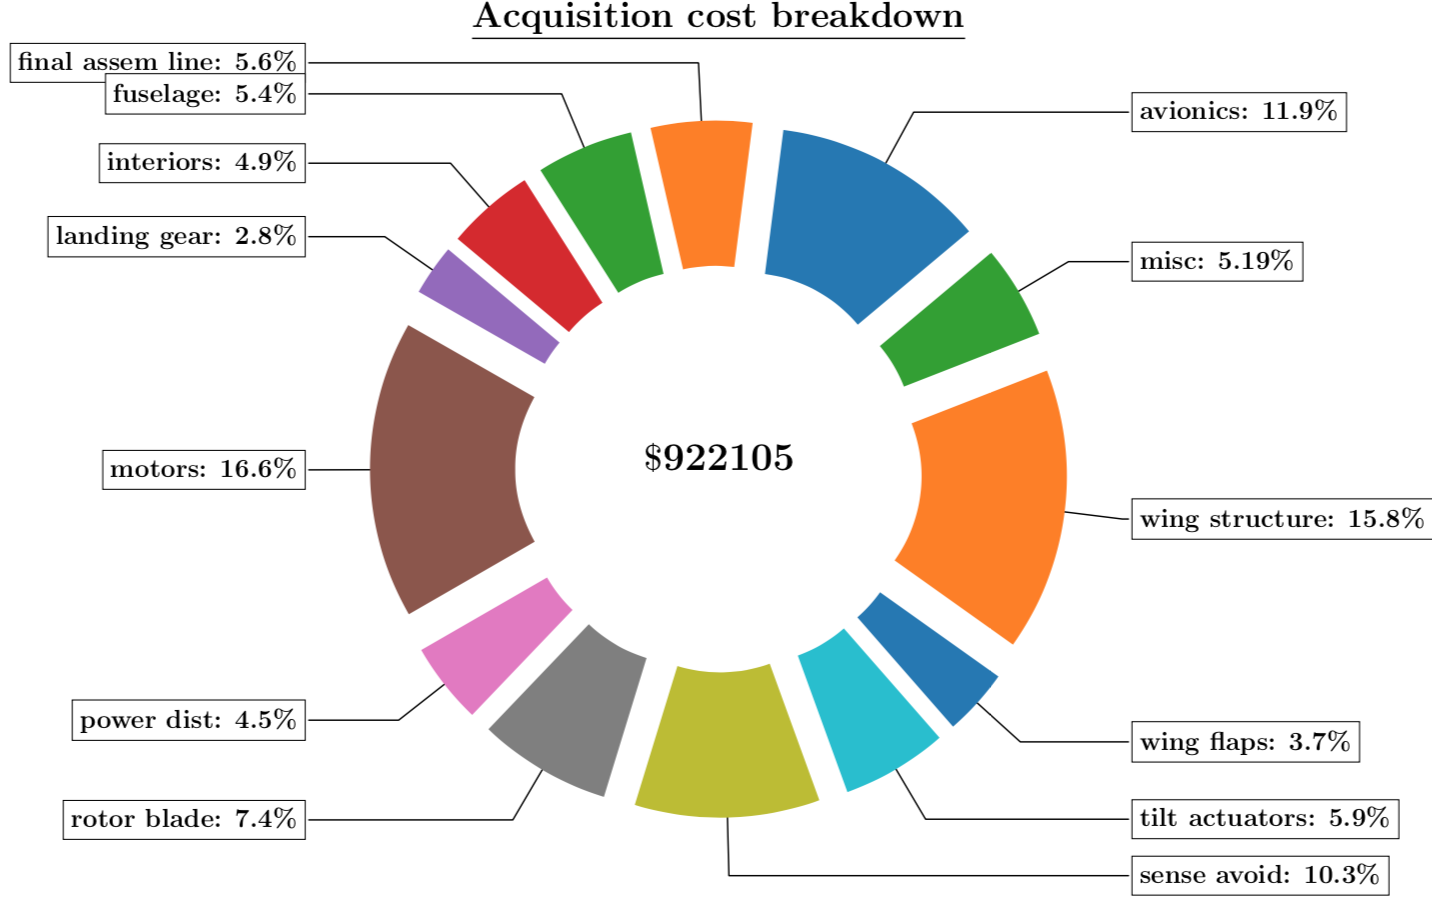
\includegraphics[width=0.45\textwidth]{images/pie3.png}}
	\subfigure[Annual cost]{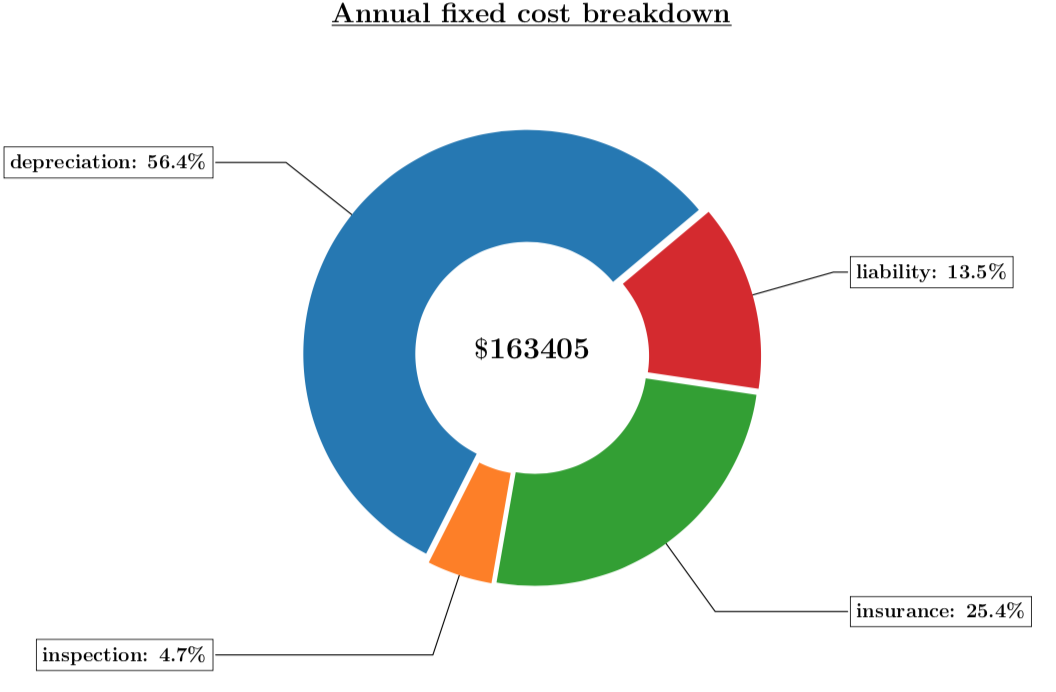
\includegraphics[width=0.45\textwidth]{images/pie5.png}}
	\subfigure[Operating cost]{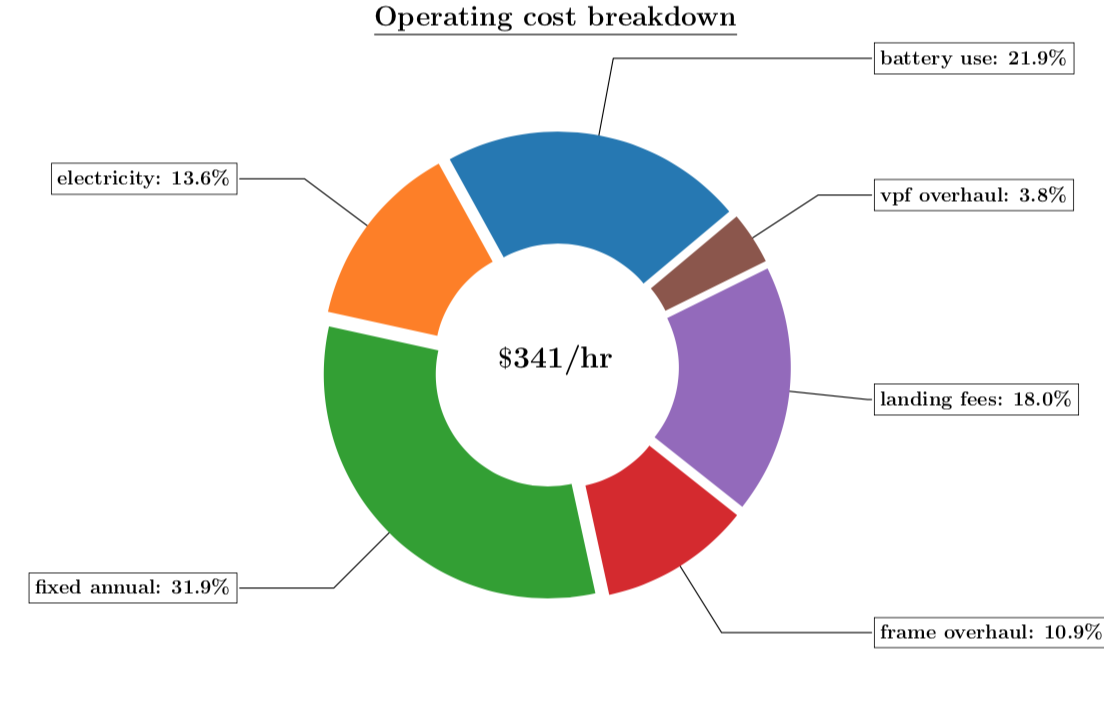
\includegraphics[width=0.45\textwidth]{images/pie2.png}}
	\subfigure[Parasitic drag breakdown]{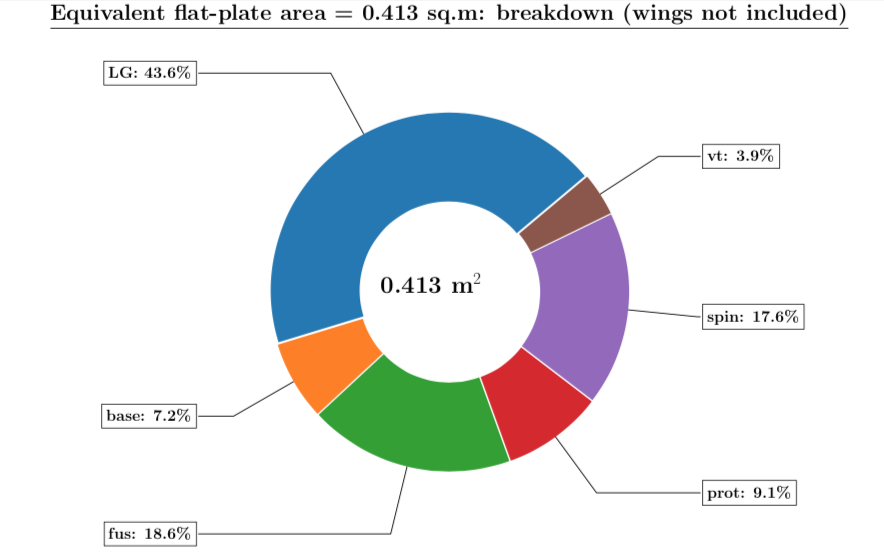
\includegraphics[width=0.45\textwidth]{images/pie1.png}}
	\subfigure[Vehicle weight]{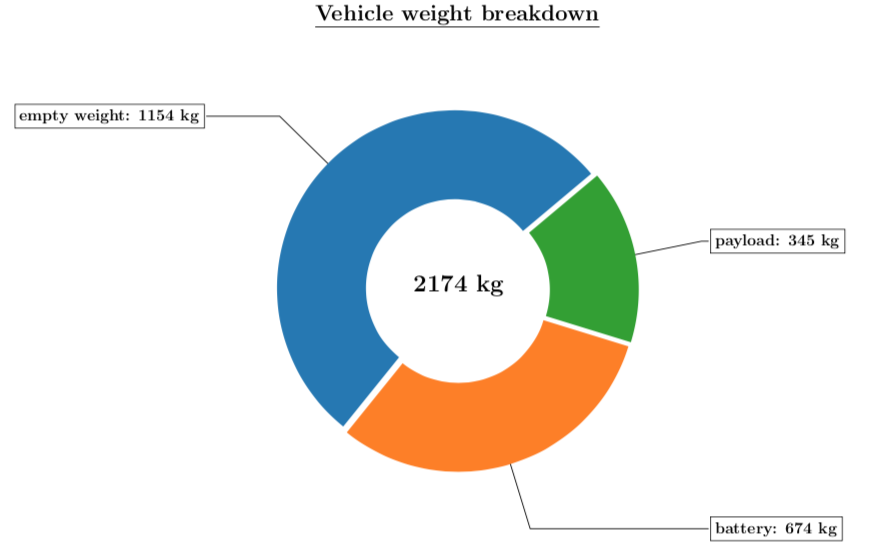
\includegraphics[width=0.45\textwidth]{images/pie6.png}}
	\subfigure[Empty weight]{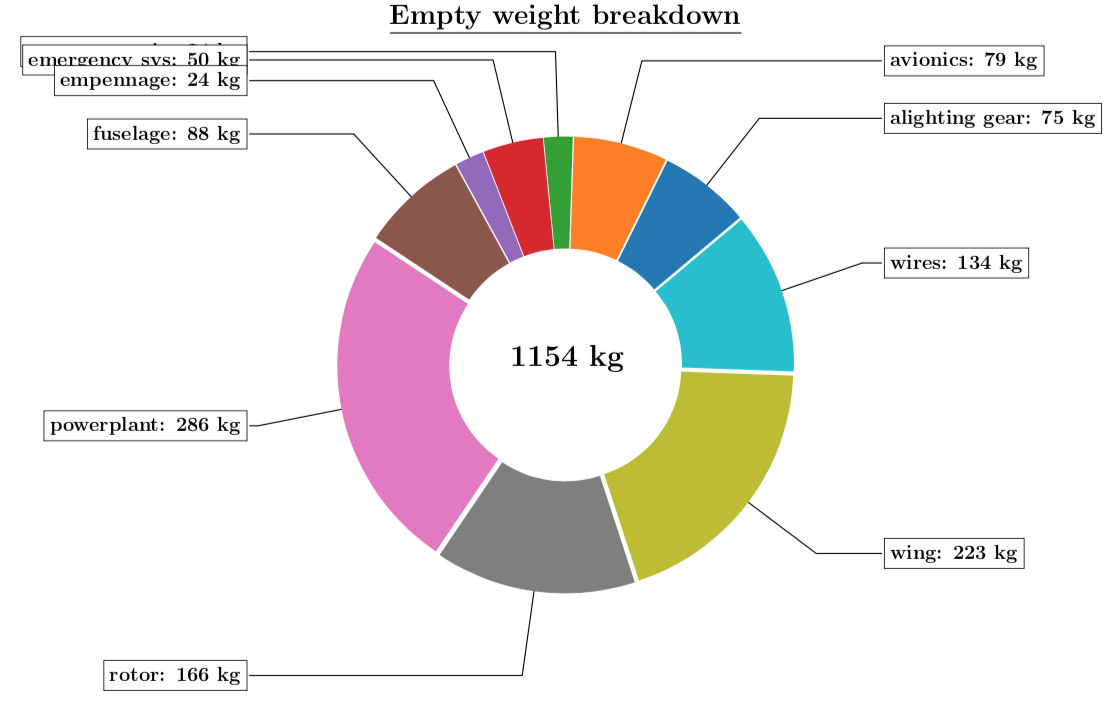
\includegraphics[width=0.45\textwidth]{images/pie7.png}}
     \caption{Pie charts generated by piethon.py postprocessor for a single design}
     \label{fig:pies}
\end{figure}

\item \textbf{Battery charge profile}: \hydra \spc features the ability to visualize the battery state of charge as a function of time along the mission profile. This postprocessor can be invoked with the command 
\begin{center}
\textbf{python3 Postprocessing/battery\_draw.py 10}
\end{center}
Here, 10 is the unique design ID for the sized vehicle that needs to be postprocessed. The resulting plot is stored in a PDF called \textbf{battery\_design\_10.pdf}, and shown in Fig.~\ref{fig:battery_profile}. The first subplot shows the estimated vehicle range for a ``perfect battery'' starting the mission at its theoretical maximum state of charge. The second subplot shows the same ``ideal battery'' charge, along with the estimated battery state of charge used in \hydra \spc for sizing the vehicle.

\begin{figure}
     \centering
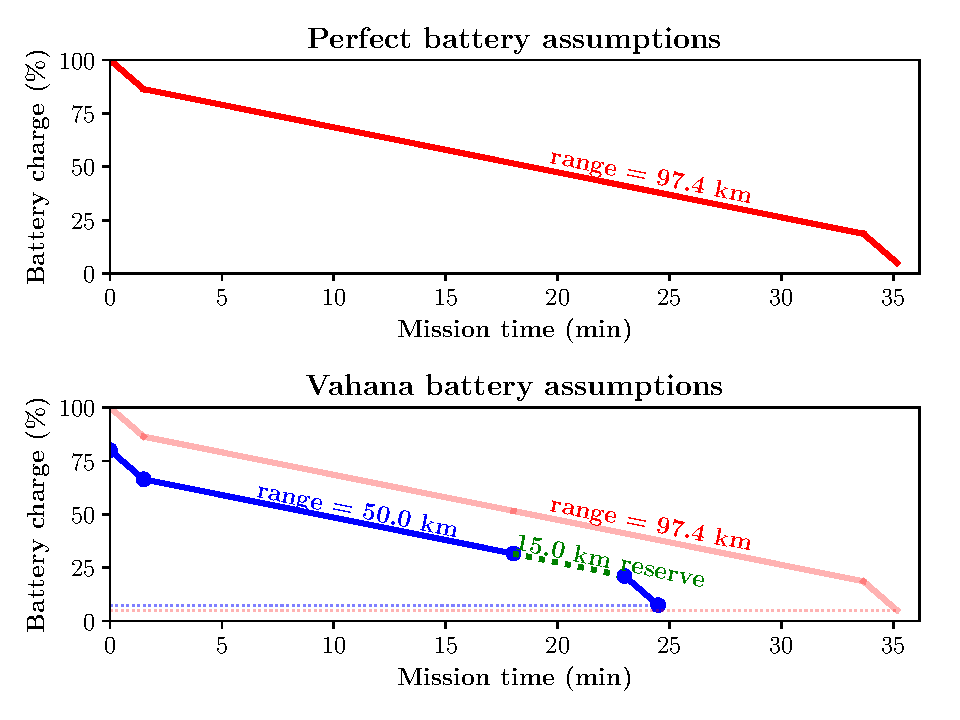
\includegraphics[width=0.9\textwidth]{images/battery_design_10.pdf}
\caption{Battery state of charge along mission profile}
\label{fig:battery_profile}
\end{figure}

\item \textbf{Vehicle performance}: To automatically generate the (approximate) power curve, payload-range and payload-endurance trade offs, \hydra \spc features a performance postprocessor that can be invoked as follows:
\begin{center}
\textbf{python3 Postprocessing/performance.py 28}
\end{center}
Here, 28 is the unique design identifier that will be analyzed at various airspeeds and longitudinal trim will be performed. The outputs from the postprocessor are shown in the following pages.

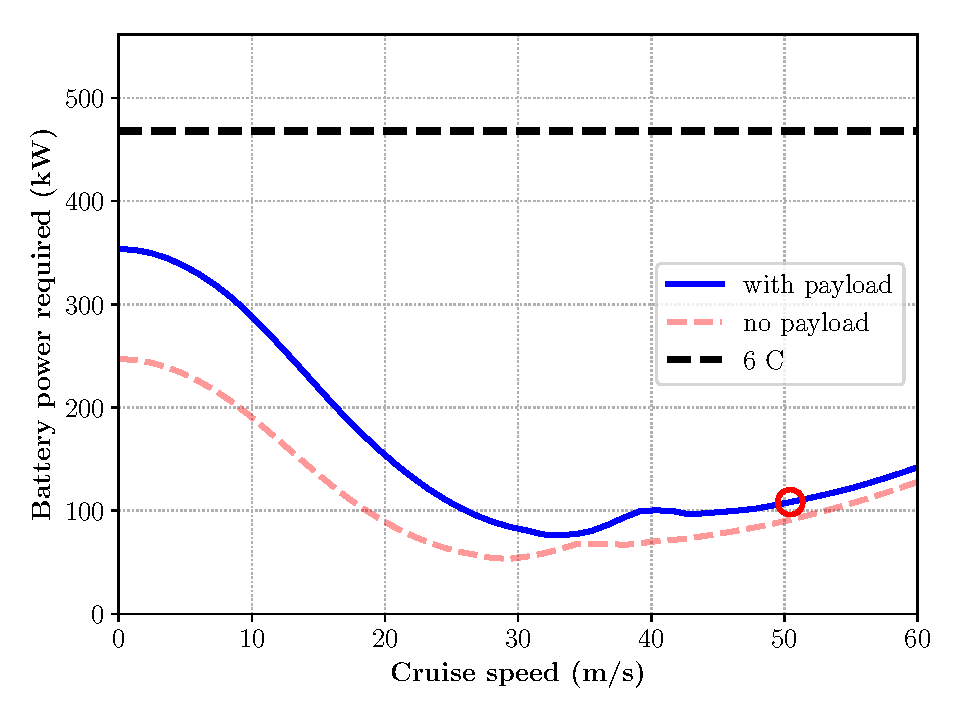
\includepdf[pages={1-}]{images/performance_design_28.pdf}

\item \textbf{Sensitivity analysis}: single and two-perturbation sensitivity studies can be launched using the following script:
\begin{center}
\textbf{python3 Postprocessing/sensitivity\_wrapper.py 32}
\end{center}
Here, 32 is the unique identifier for a converged vehicle design. The resulting plots from the sensitivity of the converged design to perturbations in target airspeed (for the same mission range) are shown in the first two plots. The next four plots show the effect of changing the cruise wing loading and aspect ratio on vehicle take-off mass, installed power, battery power and operating cost as contour plots, with carpet axes. The baseline design point is marked as a circle, and invalid designs are marked with a red cross (\red{$\times$}) inside a gray circle \textcolor{gray}{$\mathlarger{\circ}$}. The final two plots show the effect of changing the rotor hover blade loading and hover tip speed on take-off mass, installed power, battery mass and operating cost. These results are stored in a PDF named sensitivities\_design\_32.pdf.

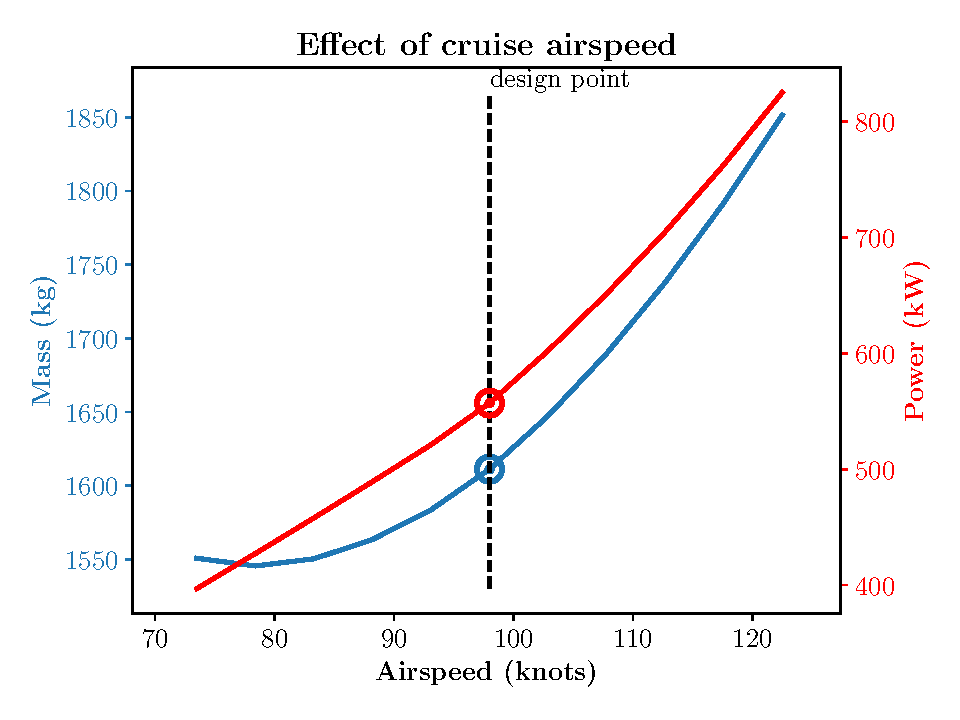
\includepdf[pages={1-}]{images/sensitivities_design_32.pdf}

\item \textbf{Optimization}: After running \textbf{xrun.py}, use the following commands to invoke sizing optimization:
\begin{flushleft}

\textbf{python3 process\_data.py}  \qquad  \#$\Rightarrow$ filter out invalid designs, rank\\
\textbf{python3 Postprocessing/optimize\_driver.py} \qquad \# serial mode\\
\textbf{mpirun -n 8 python3 Postprocessing/optimize\_driver.py} \# parallel
\end{flushleft}

This command launches two types of optimization: (a) gradient-based optimization (several threads), with several initial conditions based on valid designs identified by the \textbf{process\_data.py} command, and (b) differential evolution (first thread), with a latin-hypercube initial sampling. The optimized designs (generated by both methods) are aggregated and checked for uniqueness and validity. These unique designs are written to the file \textbf{optim\_summary.dat}, with the syntax identical to \textbf{summary.dat} and \textbf{best\_design.dat}. Additionally, the file \textbf{optim\_dvars\_summary.dat} shows the values of the design variables that yield the optimum design. After optimization is complete, the outputs/log/ folder will feature files with the pattern \textbf{optim\_log\_<XYZ>.yaml} and \textbf{optim\_log\_<XYZ>.txt}, with patterns similar to the regular output files of the same format. The process\_data.py command can be called with an additional argument `optim' as follows:
\begin{center}
\textbf{python3 process\_data.py optim}
\end{center}
This command sorts the various optimized unique designs in \textbf{optim\_summary.dat} from best to worst and writes the results in a file called \textbf{optim\_ranked.dat}.

\end{enumerate}